\chapteropen{Chapter 3: Use-case modelling}{chapter-3}
\markboth{Ch. 3 | Use cases}{}


\begin{studycolumns}
\vspace{0pt}
\begin{eli5box}
A use case is a promise about a user's goal, like 'borrow a book'. An actor is a role standing outside the system. The diagram is the menu of goals; the description is the recipe showing what the user and system do, including what happens when something goes wrong.
\end{eli5box}
\textbf{Answer check:} Start with the boundary and external roles; name goals, then describe actor/system steps and alternatives. Include is required reuse; extend is conditional extra behaviour. Neither means ``happens next. Authentication may be a precondition without a fresh login each time. Keep denial/conflict paths inside the behaviour when they must be explained.
\needspace{4\baselineskip}
\subsection*{Visual: decide between include and extend}
\sectionlabel{h-visual-decide-between-include-and-extend}
First identify a meaningful unit of behaviour; do not turn every sentence into a use case.
\end{studycolumns}


\par\smallskip\noindent\begin{minipage}{\linewidth}\centering
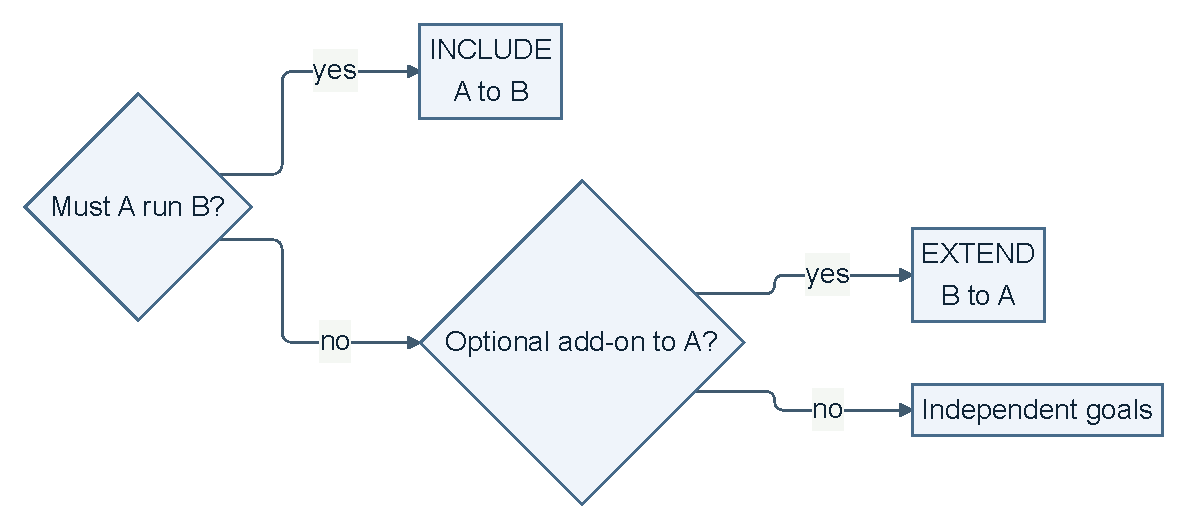
\includegraphics[width=349.60pt]{images/fig-004.pdf}
\captionof{figure}{decide between include and extend}\end{minipage}\par\smallskip

\begin{studycolumns}
\vspace{0pt}



\needspace{4\baselineskip}
\subsection*{3.1 UML in one table}
\sectionlabel{h-31-uml-in-one-table}
UML = \emph{a graphical notation with textual annotation for specifying, documenting and communicating structure, functionality and dynamic behaviour of complex software systems.} Booch + Jacobson + Rumbaugh; the lecture gives UML 1.1 adoption in 1997 and refers to UML 2.5 (2015). These are historical references in the supplied slides, not a claim about the current UML release.


\begin{referenceentries}
\textit{\textbf{Category} / \textbf{Diagrams}}\par\smallskip
\noindent \textbf{\textbf{Structure} (static, "irrespective of time")}: Class, Object, Package, Component, Composite Structure, Deployment (L3 list)\par
\noindent \textbf{\textbf{Behaviour} (dynamic)}: \textbf{Use Case}, \textbf{Activity}, \textbf{State Machine}, \textbf{Sequence}, \textbf{Communication}, Interaction Overview, Timing\par
\end{referenceentries}
Course modelling focus: \textbf{use case, class, sequence, state machine, activity} (communication/\allowbreak{}object appear in the SRS figure list).

\textbf{Trap:} UML is \textbf{not} a programming language and \textbf{not} a method. "Only use the diagrams that are useful and necessary to define the system" --- select diagrams for the modelling need rather than drawing every diagram type.

\needspace{4\baselineskip}
\subsection*{3.2 Use case model = static + dynamic}
\sectionlabel{h-32-use-case-model--static--dynamic}

\begin{quote}\small\color{navy}
\textbf{Use case model = Use case diagram (static) + Use case descriptions (dynamic).}

\end{quote}
The diagram identifies relationships; the description specifies the behaviour. Supply both when requested.
\end{studycolumns}

\Needspace{4\baselineskip}
\subsection*{3.3 Diagram elements}
\sectionlabel{h-33-diagram-elements}


{\fontsize{9}{11}\selectfont
\begin{longtable}{L{\dimexpr 0.22801\linewidth-5.47pt\relax}L{\dimexpr 0.36291\linewidth-8.71pt\relax}L{\dimexpr 0.40908\linewidth-9.82pt\relax}}
\toprule
\rowcolor{ice}\textbf{Element} & \textbf{Notation} & \textbf{Meaning} \\
\midrule\endfirsthead
\toprule\rowcolor{ice}\textbf{Element} & \textbf{Notation} & \textbf{Meaning} \\
\midrule\endhead
\multicolumn{3}{r}{\scriptsize Continued on next page}\\\endfoot
\bottomrule\endlastfoot
\textbf{Actor} & Stick figure, labelled with role (not a person's name) & An \textbf{external} entity that interacts with the system \\
\textbf{Use case} & Ellipse, labelled with a verb phrase & A unit of functionality performed by the system yielding a result/\allowbreak{}value for an actor \\
\textbf{Association} & Solid line actor\ensuremath{\leftrightarrow}use case & Actor participates in that use case \\
\textbf{System boundary} & Rectangle around use cases & Separates system from environment \\
\textbf{Generalization} & Solid line, hollow triangle pointing to the parent & Actor or use-case specialisation \\
\textbf{\guillemotleft{}include\guillemotright{}} & Dashed arrow from base \ensuremath{\rightarrow} included & Base \textbf{always} performs the included behaviour \\
\textbf{\guillemotleft{}extend\guillemotright{}} & Dashed arrow from extending \ensuremath{\rightarrow} base & Extending behaviour is \textbf{optional/\allowbreak{}conditional} \\
\end{longtable}
}


\Needspace{4\baselineskip}
\subsection*{3.4 \guillemotleft{}include\guillemotright{} vs \guillemotleft{}extend\guillemotright{} --- decomposition, reuse and optional behaviour}
\sectionlabel{h-34-include-vs-extend--decomposition-reuse-and-optional-behaviour}


{\fontsize{9}{11}\selectfont
\begin{longtable}{L{\dimexpr 0.22236\linewidth-5.34pt\relax}L{\dimexpr 0.43297\linewidth-10.39pt\relax}L{\dimexpr 0.34467\linewidth-8.27pt\relax}}
\toprule
\rowcolor{ice}\textbf{} & \textbf{\textbf{\guillemotleft{}include\guillemotright{}}} & \textbf{\textbf{\guillemotleft{}extend\guillemotright{}}} \\
\midrule\endfirsthead
\toprule\rowcolor{ice}\textbf{} & \textbf{\textbf{\guillemotleft{}include\guillemotright{}}} & \textbf{\textbf{\guillemotleft{}extend\guillemotright{}}} \\
\midrule\endhead
\multicolumn{3}{r}{\scriptsize Continued on next page}\\\endfoot
\bottomrule\endlastfoot
Trigger & Always, as part of the base & Under an explicit condition /\allowbreak{} at an extension point \\
Purpose & Functional decomposition, or \textbf{reuse} of common behaviour & Add \textbf{optional} functionality \\
Base alone is\ldots{} & \textbf{Incomplete} without the included UC & \textbf{Complete by itself} \\
Arrow direction & base ----\ensuremath{\blacktriangleright} included & extending ----\ensuremath{\blacktriangleright} base \\
Course example & Manage Incident \textbf{includes} Create /\allowbreak{} Handle /\allowbreak{} Close Incident; Open Incident and Allocate Resources \textbf{include} View Map & Report Emergency \ensuremath{\blacktriangleleft}---- \textbf{extends} ---- Help \\
\end{longtable}
}

\begin{studycolumns}
\vspace{0pt}


\begin{quote}\small\color{navy}
\textbf{Trap \#1 (arrow direction).} Students reverse \guillemotleft{}extend\guillemotright{} arrows constantly. Mnemonic: \textbf{"include points to the helper; extend points to the host."}

\textbf{Trap:} conditional behaviour can remain an alternative/exception flow. Use extend only for a separate optional unit; required reused behaviour uses include.


\end{quote}
\needspace{4\baselineskip}
\subsection*{3.5 The use case description --- mandatory fields}
\sectionlabel{h-35-the-use-case-description--mandatory-fields}
\begin{enumerate}
\item \textbf{Participating actors} (with the \textbf{initiating actor} identified).
\begin{itemize}
\item A use case can have more than one participating actor.
\item The \textbf{initiating actor triggers} the use case.
\item If triggered by a \textbf{system event or another use case}, the initiating actor is \textbf{NULL}.
\end{itemize}
\item \textbf{Entry conditions (pre-condition)} --- system state that must be satisfied to execute.
\item \textbf{Exit conditions (post-condition)} --- system state that must be reached afterwards.
\item \textbf{Flow of events} (a.k.a. normal /\allowbreak{} main success flow) --- alternating actor and system steps: step 1 = how the actor triggers; step 2 = how the system responds; \ldots{}
\item \textbf{Alternative flows} --- variations or errors that \textbf{return to the normal flow} (e.g. invalid card/\allowbreak{}PIN \ensuremath{\rightarrow} back to step 2; insufficient funds \ensuremath{\rightarrow} back to step 6).
\item \textbf{Exceptions} --- exceptional situations that \textbf{cause the use case to fail} (e.g. three invalid PIN attempts \ensuremath{\rightarrow} card suspended; ATM out of funds \ensuremath{\rightarrow} refuses card).
\end{enumerate}
Template also captures: Use Case ID, Name, Created/\allowbreak{}Updated by, dates, Actor, Description, Priority, Frequency of Use, Includes, Special Requirements, Assumptions, Notes and Issues.

\needspace{4\baselineskip}
\subsection*{3.6 Worked example --- "Withdraw Money using ATM"}
\sectionlabel{h-36-worked-example--withdraw-money-using-atm}
\textbf{Participating actors:} Bank Customer (\textbf{initiating}), Bank (secondary/\allowbreak{}external system). \textbf{Entry conditions:} (1) customer has an account with the bank \textbf{and} (2) has an ATM card and PIN. \textbf{Exit conditions:} (1) customer receives the requested cash \textbf{or} (2) customer receives an explanation from the ATM why cash could not be dispensed.

\textbf{Normal flow (note the A/\allowbreak{}S alternation):}
\end{studycolumns}


{\fontsize{9}{11}\selectfont
\begin{longtable}{L{\dimexpr 0.14850\linewidth-3.56pt\relax}L{\dimexpr 0.35357\linewidth-8.49pt\relax}L{\dimexpr 0.49793\linewidth-11.95pt\relax}}
\toprule
\rowcolor{ice}\textbf{\#} & \textbf{Actor step} & \textbf{System step} \\
\midrule\endfirsthead
\toprule\rowcolor{ice}\textbf{\#} & \textbf{Actor step} & \textbf{System step} \\
\midrule\endhead
\multicolumn{3}{r}{\scriptsize Continued on next page}\\\endfoot
\bottomrule\endlastfoot
1 & Inputs the card into the ATM &  \\
2 &  & Requests input of a six-digit PIN \\
3 & Enters a PIN &  \\
4 &  & Verifies card and PIN with account info in the Bank \\
5 &  & If verified, requests the amount to withdraw \\
6 & Enters an amount &  \\
7 &  & Verifies the amount is available in the account \\
8 &  & If sufficient funds, outputs money, card and receipt \\
9 & Removes card, receipt and money &  \\
\end{longtable}
}

\begin{studycolumns}
\vspace{0pt}

\textbf{Alternative flows}

\begin{itemize}
\item \textbf{AF-S5 (invalid card and PIN):} 1. ATM displays "Invalid card and PIN. Please try again!" for 2 s. 2. ATM \textbf{returns to step 2}.
\item \textbf{AF-S8 (insufficient funds):} 1. ATM displays "Insufficient funds\ldots{} enter a smaller amount!" for 2 s. 2. ATM \textbf{returns to step 6}.
\end{itemize}
\textbf{Exceptions}

\begin{itemize}
\item \textbf{EX1 (invalid PIN three times):} 1. Displays "Card is suspended! Please call customer service (1633)\ldots{}" for 2 s. 2. Outputs the card. \ensuremath{\rightarrow} \emph{Use case fails.}
\item \textbf{EX2 (ATM has insufficient funds):} 1. Displays "This ATM is off-service due to insufficient funds!" at the start screen. 2. Does not accept the card.
\end{itemize}

\begin{quote}\small\color{navy}
\textbf{Trap:} the AF/\allowbreak{}EX distinction is graded. \textbf{AF = recoverable, returns to a step. EX = terminal, the goal is not achieved.} "Insufficient funds in \emph{account}" is recoverable (AF); "insufficient funds in \emph{ATM}" is not (EX). Read carefully which one the question describes.

\end{quote}
\needspace{4\baselineskip}
\subsection*{3.7 Deriving use cases from functional requirements}
\sectionlabel{h-37-deriving-use-cases-from-functional-requirements}
Use the Library Management System drill (L3):
\end{studycolumns}


{\fontsize{9}{11}\selectfont
\begin{longtable}{L{\dimexpr 0.07599\linewidth-3.04pt\relax}L{\dimexpr 0.33209\linewidth-13.28pt\relax}L{\dimexpr 0.21261\linewidth-8.50pt\relax}L{\dimexpr 0.19839\linewidth-7.94pt\relax}L{\dimexpr 0.18092\linewidth-7.24pt\relax}}
\toprule
\rowcolor{ice}\textbf{\#} & \textbf{Functional requirement} & \textbf{Actor(s)} & \textbf{Use case} & \textbf{Association} \\
\midrule\endfirsthead
\toprule\rowcolor{ice}\textbf{\#} & \textbf{Functional requirement} & \textbf{Actor(s)} & \textbf{Use case} & \textbf{Association} \\
\midrule\endhead
\multicolumn{5}{r}{\scriptsize Continued on next page}\\\endfoot
\bottomrule\endlastfoot
1 & Member searches for materials & Member & Search Material & --- \\
2 & Member loans materials & Member & Loan Material & --- \\
3 & System verifies membership with University Account System \textbf{before} loan & Member, University Account System & Verify Member & \guillemotleft{}include\guillemotright{} from Loan Material \\
4 & Member returns materials via drop-off kiosk & Member, Library Drop-off Kiosk & Return Material & --- \\
5 & System sends overdue notice via CITS Email Server & CITS Email System & Send Overdue Notice & --- \\
6 & \textbf{When} network to CITS fails, log the event & --- (system event) & Log Network Issues & \guillemotleft{}extend\guillemotright{} on Send Overdue Notice \\
\end{longtable}
}

\begin{studycolumns}
\vspace{0pt}

\textbf{Method (do this in the exam, in order):}

\begin{enumerate}
\item \textbf{Identify actors} --- scan for \emph{people/\allowbreak{}roles} and \emph{external systems}; underline nouns.
\item \textbf{Identify use cases} --- scan for \emph{verb phrases describing a goal} ("search", "loan", "return", "send notice"). One goal = one use case.
\item \textbf{Identify associations} --- draw actor\ensuremath{\leftrightarrow}UC lines only where the actor participates.
\item \textbf{Add include/\allowbreak{}extend/\allowbreak{}generalization} --- only where justified; annotate with one sentence of reasoning.
\item \textbf{Write the description} for the use cases the question names.
\end{enumerate}
\textbf{Lecture comparison.} L3, pp. 20--22, shows three candidate library diagrams, including different choices of actor and authentication behaviour. Do not treat every candidate as an approved solution. Trace each element to the stated requirements: membership verification is required before a loan; Login is not stated for the library example. L4, pp. 12--16, separately uses Login in the course registration example. Explain the system boundary and reuse choice.

\textbf{Trap --- actors vs system internals.} "Database", "Sensor" (if part of the system's own hardware), "UI" are \textbf{not} actors. But an \textbf{external} University Account System, CITS Email Server, Billing System, Library Drop-off Kiosk \textbf{are} actors.

\textbf{Trap --- actor generalization.} If Student and Professor share Login, model an abstract \textbf{User} actor with generalization arrows from Student/\allowbreak{}Professor to User, then associate Login with User. Do not draw duplicate Logins.
\end{studycolumns}
